\chapter{Statistical Analysis}
    \label{ch:stat}

	The statistical analysis of results is done via a Bayesian approach where first a search for signs of new physics is done with a calculation of the significance of any excesses. Then in the absence of a signals exclusion limits on the scale of new physics (either $\Lambda$ or M$_{s}$) are set. A slightly different search approach is made between CI and ADD. In CI the shape of new physics is studied and therefore a series of invariant mass search bins are used with bin edges of 400, 550, 800, 1200, 1800, 3000 and 4500 GeV. With the addition of information from the $\cos{\theta^{*}}$ variable in this analysis bins are also then split up in $\cos{\theta^{*}}$ as well as invariant mass. As seen in section \ref{sec:binOpp} most of the new information is obtained via using two bins in $\cos{\theta^{*}}$ making a total of 12 search bins distributed in invariant mass and $\cos{\theta^{*}}$. ADD on the other hand cannot use the many search bin approach due to a sharper turn-on and undefined nature of the signal after the cut-off point. Therefore only one search bin is used to search for ADD with a minimum invariant mass cut of 1900 GeV and upper cut of 4500 GeV. The lower range of this search bin is optimised by choosing the value with the highest expected limit. The ADD model gains no additional discriminating power from the $\cos{\theta^{*}}$ variable. For each search bin a parametrisation of new physics is produced (discussed in section \ref{sec:parm}) as well as the background predicted and data observed. Also included is the background and signal parametrisation varied by each of the appropriate sources of systematic error (discussed in section \ref{sec:sys}) for signal and background. This all composes the input to the statistical analysis. 


    The statistical analysis is carried out using the ROOT \cite{Antcheva20092499} package BAT or Bayesian Analysis Tool-kit \cite{Caldwell20092197}. This package allows for the integration over nuisance parameters (discussed below) using the Markov Chain Monte Carlo method.  The statistical analysis starts off with the definition of the number of expected events $\mu$ found in the signal region as seen in equation \ref{eq:bay_events}.

	\begin{equation}
		\mu = n_{s}(\Theta,\overline{\Omega}) + n_{b}(\overline{\Omega})
    	\label{eq:bay_events}
    \end{equation}

    Here $n_{s}$ is the number of signal events predicted by the model with a particular model parameter $\Theta$ and $n_{b}$ is the total number of predicted background events. $\overline{\Omega}$ is then a set of Gaussian nuisance parameters or systematic uncertainties on the number of expected events for signal and background. A product of Poisson probabilities for each search bin $k$ gives the Bayesian likelihood, seen in equation \ref{eq:likelihood}, of observing $n$ events given the signal parameter $\Theta$ and nuisance parameters $\overline{\Omega}$.

	\begin{equation}
		\mathcal{L}(n~|~\Theta,\overline{\Omega}) = \prod\limits^{N}_{k=1}{\frac{\mu^{n_{k}}_{k} e^{-\mu_{k}}}{n_{k}!}}
    	\label{eq:likelihood}
    \end{equation}

    where $\mu^{n_{k}}_{k}$ and $n_{k}$ are the total number of expected events and observed number of events in search bin $k$ respectively. 


	\begin{equation}
		\mathcal{P}(\Theta~|~n) = \frac{1}{\mathcal{Z}}\mathcal{L}_{\mathcal{M}}(n~|~\Theta)P(\Theta)
    	\label{eq:postProb}
    \end{equation}

    Equation \ref{eq:postProb} shows the posterior probability using Bayes' theorem for the observation of $\Theta$ given $n$. Here $\mathcal{Z}$ is the normalisation factor and $\mathcal{L}_{\mathcal{M}}$ is the marginalised likelihood after all nuisance parameters have been integrated out. It is assumed all nuisance parameters are correlated across all search bins. A full description of nuisance parameters can be found in section \ref{sec:sys}. Finally $P(\Theta)$ is the prior probability of $\Theta$. A 95\% confidence level (CL) limit can then be found by finding $\Lambda_{lim}$ that satisfies $\int_{0} ^{\theta_{lim}} P(\theta~|~\bar{n}) d\theta = 0.95$. For CI $P(\Theta)$ is chosen to be uniform and positive with respect to $1/\Lambda^{2}$ or $1/\Lambda^{4}$. This form of priors is chosen due to the form of differential cross-section (equation \ref{eq:DiffCross}) and its dependence on $\Lambda$. It is not obvious which prior is more correct as these forms refer to the interference and pure CI terms respectively which change in dominance throughout the search bins and model parameters, therefore the search is done using both parameters for completeness. A similar effect is seen in the form of the ADD differential cross-section (equation \ref{eq:ADDcs}) and so there a prior of $1/M_{s}^{4}$ or $1/M_{s}^{8}$ is used for the same reason. 

    In order to check all signal formalisms 1000 background-like Pseudo-Experiments (PE) are run using BAT for each formalism. Each PE is then passed through the Bayesian statistical method above so they can be compared to data and signal predictions. Figure \ref{fig:pdf_CI_main} shows posterior probability density functions (pdf's), for two CI formalisms, of these 1000 PE's.

    \begin{figure}[h]
        \begin{center}
            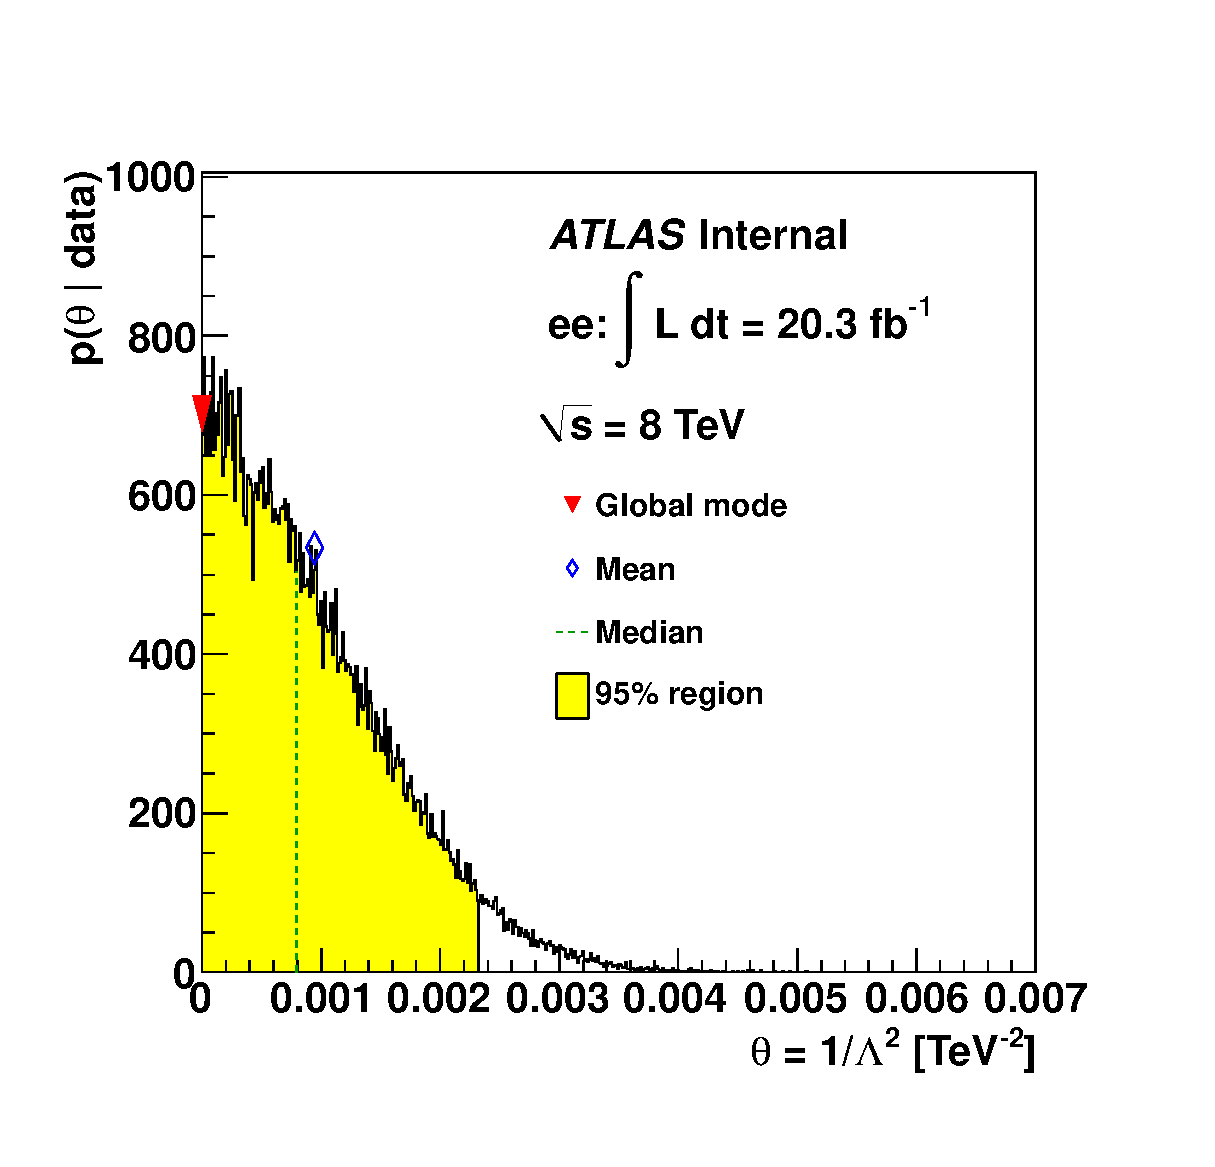
\includegraphics[width=0.49\linewidth]{images/post_LL_minus.eps}
            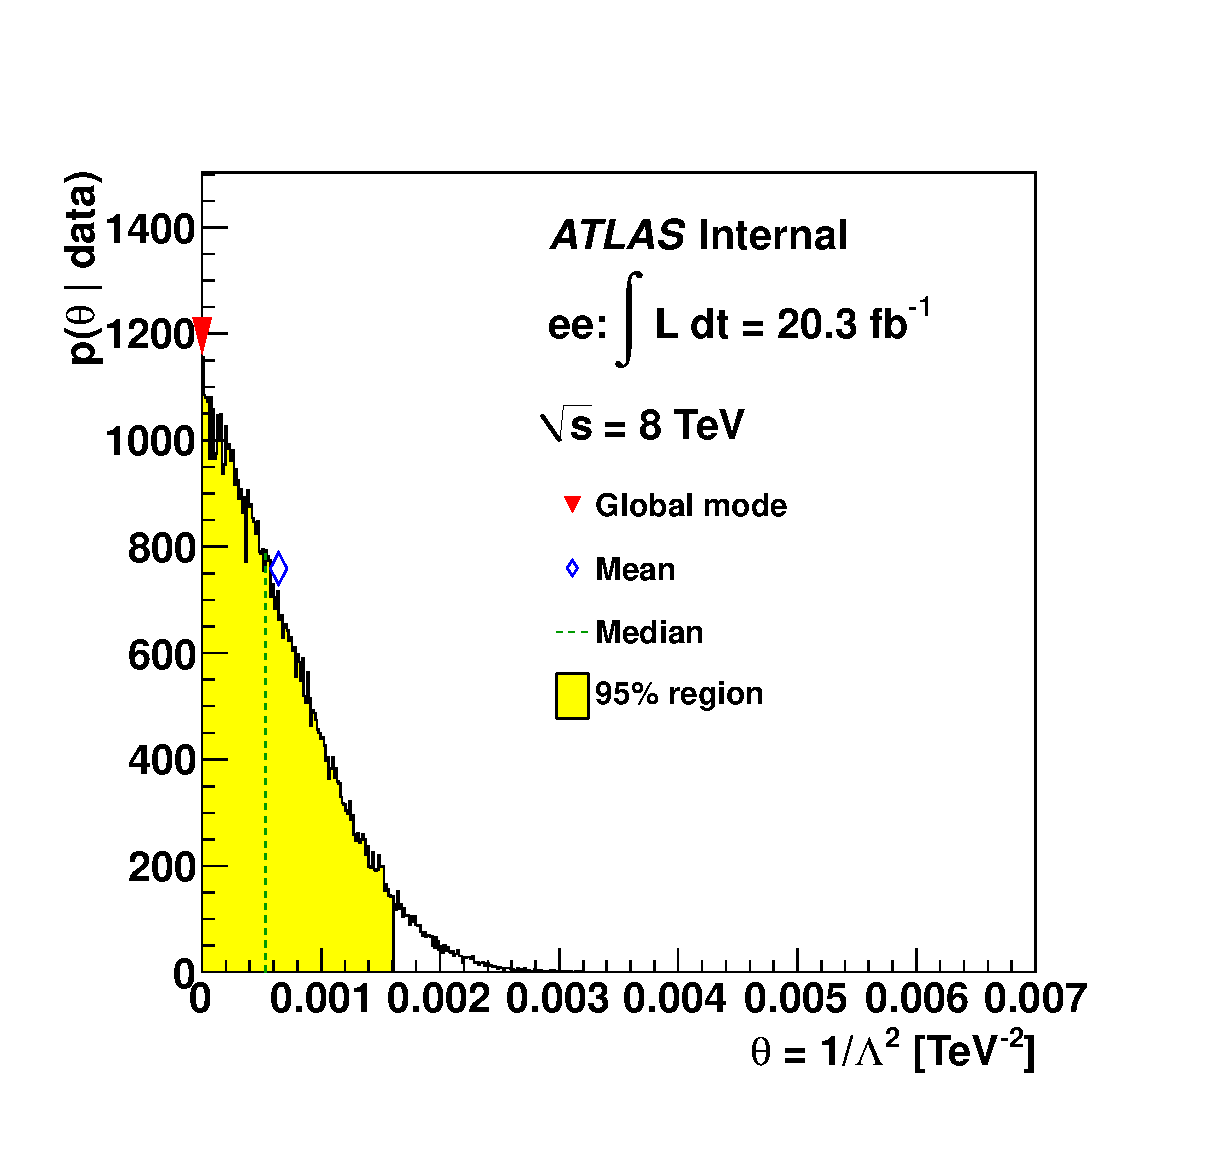
\includegraphics[width=0.49\linewidth]{images/post_LR_minus.eps}
        \end{center}
       \caption{Posterior pdf distributions for the CI model formalisms LL and LR with constructive interference and a uniform positive prior in $1/\Lambda^{2}$.}
       \label{fig:pdf_CI_main}
    \end{figure}

    % \begin{figure}[h]
    %     \begin{center}
    %         %\includegraphics[scale=0.6,natwidth=610,natheight=642,angle=-90]{images/}
    %     \end{center}
    %    \caption{Posterior pdf distributions for the ADD model with a uniform positive prior in $1/M_{s}^{8}$.}
    %    \label{fig:pdf_ADD_main}
    % \end{figure}



\section{Systematics}
    \label{sec:sys}

    The list of nuisance parameters used for this statistical analysis make up a list of all systematic errors considered as relevant for this analysis. Table \ref{tab:sys} lists all the systematic errors used for this analysis along with their size while figures \ref{fig:invMass_main}, \ref{fig:AFB_main} and \ref{fig:cosTS_main} in the previous chapter show total background systematic errors in their ratio's. 
    Due to this analysis using both the forward and backwards regions in the search all systematics needed to be assessed for both these regions separately.
    Following is a brief description of each of the systematics including how they were derived.

    \begin {table}[h]
        \begin{center}
        \begin{tabular}{ | l | c c | } 
            \hline
            \multirow{2}{*}{Source} & \multicolumn{2}{c|}{Signal Systematic [\%]}               \\
                                & Forward                           & Backward                        \\
            \hline
            Normalization       & 4.0 ~(4.0) ~[4.0]           & 4.0 ~(4.0) ~[4.0]         \\
            PDF Variation       & $<$ 0.1 ~(0.2) ~[0.5]       & $<$ 0.1 ~(0.2) ~[0.5]     \\
            PDF Choice          & NA                                & NA                              \\
            $\alpha_S$          & NA                                & NA                              \\
            EW Corrections      & $<$ 0.1 ~($<$ 0.1) ~[0.1]   & $<$ 0.1 ~($<$ 0.1) ~[0.1] \\
            Photon-Induced      & NA                                & NA                              \\
            Efficiency          & 1.0 ~(2.0) ~[3.0]           & 1.0 ~(2.0) ~[3.0]         \\
            Scale/Resolution    & 1.2 ~(2.4) ~[5.0]           & 1.2 ~(2.4) ~[5.0]         \\
            Multijet/$W$+jets  & NA                                & NA                              \\
            Beam Energy         & 1.0 ~(3.0) ~[5.0]           & 1.0 ~(3.0) ~[5.0]         \\
            Charge MisID        & 1.2 ~(2.0) ~[2.9]           &  1.2 ~(2.0) ~[2.9]        \\
            Statistical         & 3.0 ~(3.0) ~[3.0]           & 3.0 ~(3.0) ~[3.0]         \\
            \hline  
            Total               & 5.5 ~(6.9) ~[9.6]             & 5.5 ~(6.9) ~[9.6]        \\
            \hline
            \hline
            \multirow{2}{*}{Source} & \multicolumn{2}{c|}{Background Systematic [\%]}          \\
                                & Forward                           & Backward                      \\
            \hline
            Normalization       & 4.0 ~(4.0) ~[4.0]           & 4.0 ~(4.0) ~[4.0] \\
            PDF Variation       & 6.0 ~(12.5) ~[35.0]         & 10.0 ~(28.0) ~[62.5] \\
            PDF Choice          & 1.0 ~(7.0) ~[22.0]          & 1.0 ~(7.0) ~[22.0] \\
            $\alpha_S$          & 1.0 ~(3.0) ~[5.0]           & 1.0 ~(3.0) ~[5.0] \\
            EW Corrections      & 1.0 ~(2.0) ~[4.0]           & 1.0 ~(2.0) ~[4.0] \\
            Photon-Induced      & 6.0 ~(10.0) ~[17.0]         & 9.5 ~(16.5) ~[29.0]    \\
            Efficiency          & 1.0 ~(2.0) ~[3.0]           & 1.0 ~(2.0) ~[3.0] \\
            Scale/Resolution    & 1.2 ~(2.4) ~[5.0]           & 1.2 ~(2.4) ~[5.0] \\
            Multijet/$W$+jets  & 3.0 ~(5.0) ~[21.0]          & 3.0 ~(5.0) ~[21.0] \\
            Beam Energy         & 1.0 ~(3.0) ~[5.0]           & 1.0 ~(3.0) ~[5.0] \\
            Charge MisID        & 1.2 ~(2.0) ~[2.9]           & 1.2 ~(2.0) ~[2.9] \\
            Statistical         & 0.5 ~(0.5) ~[0.5]           & 0.5 ~(0.5) ~[0.5] \\
            \hline   
            Total               & 10.3 ~(19.6) ~[50.6]        & 14.9 ~(34.4) ~[76.1] \\ 
            \hline
        \end{tabular}
        \caption{All sources of systematic error and their approximate size as a percentage (\%) for dielectron mass of 1 TeV (2 TeV) [3 TeV].}
        \label{tab:sys}
        \end{center}
    \end {table}


    {\bf\raggedright Normalization} - This systematic accommodates the error associated with scaling MC samples within the Z peak to avoid luminosity errors however it also protects against any other sources of mass independent error. This systematic was investigated by looking at the effect of altering scale factor to its effect on the background cross-section. \\
    {\bf\raggedright PDF Variation} - PDF variation was investigated as another source of systematic error using the set of 20 eigenvector error sets provided with the MSTW2008NNLO PDF \cite{Martin:2009iq}. These eigenvectors were organised into 4 groups, A, B, C and D, of eigenvectors with effects in similar regions of the invariant mass spectrum. These 4 groups were then used as separate nuisance parameters and applied to events based on dielectron invariant mass and $\cos{\theta^{*}}$. \\ 
    {\bf\raggedright PDF Choice} - PDF choice refers to a comparison between the effects of different PDF's on the expected events from MC. Several other NNLO PDF are looked at including CT10 but the only PDF with predictions outside of the PDF variation systematic (seen above) is ABM11 \cite{Alekhin:2013dmy} and so an additional systematic is introduced of the order of this difference. \\
    {\bf\raggedright $\pmb{\alpha_{S}}$} - A systematic is introduced to account for the uncertainty in the value $\alpha_{S}$. It is varied between the values 0.11365 and 0.12044 according to the limits in MSTW. Recalculated cross-sections give a variation in the expected background and taken as the systematic. \\
    {\bf\raggedright EW Corrections} - The EW correction is derived via the use of a different generator (MCSANC \cite{Bondarenko:2013nu}) when calculating the EW K-factor and differences between the method give the systematic. \\
    {\bf\raggedright Photon-Induced} - The MC estimate for the PI fraction is predicted to be an upper estimate and so the effect of not including this background is studied and this effect on the event yield is taken as the systematic. \\
    {\bf\raggedright Efficiency} - Systematic provided by the ATLAS electron photon performance group to accommodate the trigger and reconstruction efficiency corrections (see section \ref{sec:correc}). \\
    {\bf\raggedright Scale/Resolution} - Systematic provided by the ATLAS electron photon performance group to accommodate the energy scale and energy resolution corrections (see section \ref{sec:correc}). \\
    {\bf\raggedright Multijet/$W$+jets} - Systematic associated with the data driven multijet \& $W$+jets estimate and seen in section \ref{sec:MJerror}. It is taken as a flat 20\% on the Multijet \& $W$+jets background.\\
    {\bf\raggedright Beam Energy} - The beam energy uncertainty of the LHC 4 TeV beams is given as 0.65\% giving this uncertainty which is again analysed to see its effect on event yield. \\
    {\bf\raggedright Charge MisID} - Systematic associated with opposite sign requirement in the analysis. This error is estimated by injecting a higher fraction of charge misidentification in to the DY MC sample and looking at the effect on background prediction. This is found to have an, at most, 3\% effect at high mass. \\
    {\bf\raggedright Statistical} - Systematic error of the statistical error of each of the MC samples used to estimate background and signal. \\




    % more information about some systematics
    % add pull's ????


\section{Angular Analysis Optimisation}


This section looks at some of the issues revolving around the introduction of the angular search within $\cos{\theta^{*}}$ as well as invariant mass. First a look at the effect of the loss in selection efficiency coming from the opposite sign requirement on the sensitivity of the search. Next is then a discussion on the optimisation of the binning used to search in $\cos{\theta^{*}}$.

\subsection{Effect of the Opposite Sign Requirement on Analysis Reach}
    \label{sec:oppSign}

    The opposite sign requirement is needed to ensure that calculations of the variable $\cos{\theta^{*}}$  correctly use the particle instead of anti-particle. However the selection comes with a 7\% drop in acceptance of signal in the signal search region (see table \ref{tab:eventEff}). The important question becomes what effect this has on the sensitivity of the analysis. This is important because angular dependence was introduced for a single CI formalism LR and not predicted to strongly impact the results for other formalisms. 
    A study was done on the expected limits set by the Bayesian statistical analysis (see chapter \ref{ch:stat}) both with the opposite sign requirement introduced and without it for both a search in invariant mass only and search bins distributed in both invariant mass and $\cos{\theta^{*}}$ (called the 1D and 2D search respectively below). Table \ref{tab:limits_oppSign} show limits for all of these possibilities for both the LL and LR formalisms. It is important to bear in mind this study was done before the analysis was finalised and so the limits do not represent the final results of the analysis but are consistent enough to represent the effects we are looking at. It can be seen that the introduction of the opposite sign requirement leads to a reduction in the reach of the limits while the introduction of the 2D search bin approach greatly increases the limits for the LR formalism while regaining the lost sensitivity in the case of the LL formalism. Although no difference is seen between the angular dependence of background and the LL formalism (see figures \ref{fig:cosTS_main} and \ref{fig:AFB_main}) the 2D search approach gains some extra shape information from the extra search bins used which offsets the loss of sensitivity from the opposite sign requirement. The same was found to be true for the ADD model as the LL formalism.  


    \begin {table}[h]
        \begin{center}
        \begin{tabular}{ | c | c | c | } 
            \hline
            \hline
            Search strategy & LL & LR \\
            \hline
            1D approach no & \multirow{2}{*}{19.27} & \multirow{2}{*}{21.64} \\
            opposite sign requirement & & \\
            1D approach with & \multirow{2}{*}{18.86} & \multirow{2}{*}{21.17} \\
            opposite sign requirement & & \\
            2D approach with & \multirow{2}{*}{19.40} & \multirow{2}{*}{22.31} \\
            opposite sign requirement & & \\
            \hline
            \hline
        \end{tabular}
        \caption{Expected Limits [TeV] calculated with 600 PE's for the LL and LR constructive CI formalisms looking at the effect of the opposite sign requirement on limits and introduction of 2D limits.}
        \label{tab:limits_oppSign}
        \end{center}
    \end {table}



\subsection{Optimisation of Search Bins in $\cos{\theta^{*}}$}
    \label{sec:binOpp}

    The belief at the start of the analysis was that binning within $\cos{\theta^{*}}$ would be optimised with 2 to n evenly distributed bins, varying bins in $\cos{\theta^{*}}$ or even varying number of bins throughout invariant mass. 
    %A few possibilities were investigated early on but it was seen that most of the extra information that could be gained from the angular variable $\cos{\theta^{*}}$ was found in splitting between the forward ($\cos{\theta^{*}}$ $>$ 1) and the backwards ($\cos{\theta^{*}}$ $<$ 1) regions and therefore only using two search bins in $\cos{\theta^{*}}$. 
    This study was carried out at two different points; early on in the analysis when search bins were first discussed, then towards the end when the full analysis was almost finalized. The first study looked at expected limits for individual invariant mass bins while varying the number of $\cos{\theta^{*}}$ bins. These ``limits'' do not give an accurate estimate of final limits but are used as a guide to see the sensitivity of each binning. The results from this study can be seen in table \ref{tab:limits_binOpp} where 600 PEs are run for each individual bin combination and expected limits are extracted from these. 
    Random fluctuations in the limits are seen but are almost consistent through many of the binning structures. The highest limits found within each invariant mass bin can be seen as bold and a structure with more bins at low mass while less bins at high mass can be seen. However this structure does not gain a very big advantage over any other binning structures that could be chosen due to the small size of the differences. The study was postponed until systematics were finalised. 

    \begin {table}[h!]
        \small 
        \begin{center}
        \begin{tabular}{ |l|c|c|c|c|c|c| } 
            \hline
            \hline
            {\bf Constructive Interference} & \multicolumn{6}{c|}{Mass bins [GeV]} \\ 
            \hline
            $\cos{\theta^{*}}$ binning & 400-550 & 550-800 & 800-1200 & 1200-1800 & 1800-3000 & 3000-4500 \\
            \hline
            1 bin       & 13.7154 & 15.0867 & 17.2645 & 17.4408 & 16.8898 & 8.81322 \\
            2 even bins & 14.0608 & 15.9546 & 18.0246 & 17.9244 & {\bf17.4196} & {\bf8.82076} \\
            4 even bins & 14.0553 & 15.9607 & 18.1429 & 18.1086 & 17.2942 & 8.74857 \\
            3 even bins & {\bf14.1691} & 15.7593 & 18.0305 & {\bf18.1593} & 16.9797 & 8.8057 \\
            4 bins A    & 14.0999 & {\bf16.053}  & 18.1057 & 18.1086 & 17.1486 & 8.82008 \\
            4 bins B    & {\bf14.1655} & 16.0005 & {\bf18.3324} & 18.1146 & 17.3696 & 8.81391 \\
            5 even bins & 13.7568 & 15.8124 & 18.2437 & 18.1414 & 17.0067 & 8.7914 \\
            \hline
            \hline
            {\bf Destructive Interference} & \multicolumn{6}{c|}{Mass bins [GeV]} \\
            \hline
            $\cos{\theta^{*}}$ binning & 400-550 & 550-800 & 800-1200 & 1200-1800 & 1800-3000 & 3000-4500 \\
            \hline
            1 bin       & 8.31287 & 8.98298 & 12.5147 & 14.7194 & 15.3456 & {\bf8.52415} \\
            2 even bins & 8.87217 & 9.22688 & 12.7154 & 15.0151 & {\bf15.8282} & 8.5155 \\
            4 even bins & 8.77311 & 9.38027 & 12.7906 & {\bf15.0944} & 15.6893 & 8.49673 \\
            3 even bins & 8.94302 & 9.30384 & 12.7526 & 15.0372 & 15.4184 & 8.51457 \\
            4 bins A    & 8.98625 & 9.28697 & 12.7833 & {\bf15.0953} & 15.5823 & 8.4854 \\
            4 bins B    & 8.93035 & 9.50594 & {\bf12.8105} & 15.0585 & 15.773 & 8.42107 \\
            5 even bins & {\bf9.22944} & {\bf9.59655} & 12.7666 & 15.0764 & 15.7632 & 8.44356 \\
            \hline
            \hline
        \end{tabular}
        \caption{Expected Limits on $\Lambda$ [TeV] calculated with 600 PE's for individual mass bins while varying $\cos{\theta^{*}}$ binning to select variable search bins. The highest limits found for each invariant mass bin are shown in {\bf bold}. No systematics were included in this study. Even bins refer to bins distributed evenly in $\cos{\theta^{*}}$ while A and B refer to larger bins in the centre of the $\cos{\theta^{*}}$ distribution and larger bins at the extremes in $\cos{\theta^{*}}$ respectively while still being symmetric around $\cos{\theta^{*}}$ = 0.}
        \label{tab:limits_binOpp}
        \end{center}
    \end {table}


    The second study seen in table \ref{tab:limits_fourbin} found very quickly that while changing from a 1D to a 2D search strategy using two evenly sized bins in $\cos{\theta^{*}}$, gave a moderate increase in limits, any further increase in the number of $\cos{\theta^{*}}$ search bins gave no increase or a slight decrease in limits. This found that most of the extra information gained from searching in $\cos{\theta^{*}}$ was seen in a split between forward ($\cos{\theta^{*}}$ $>$ 0) and backwards ($\cos{\theta^{*}}$ $<$ 0) regions. The cause of this effect comes from the introduction of systematics that grow at high mass as well as the increase in MC statistical error when binning the signal in finer bins. 
    The two bin search structure was therefore chosen as optimal for searching in the $\cos{\theta^{*}}$ variable meaning that with 6 invariant mass search bins 12 total search bins are used. 

 
    \begin {table}[h]
        \begin{center}
        \begin{tabular}{ | c | c | c | } 
            \hline
            \hline
            $\cos{\theta^{*}}$ bins & Constructive & Destructive \\
            \hline
            1 bin & 21.1691 & 17.0884 \\
            2 bin & 22.3078 & 17.6309 \\
            4 bin & 22.1839 & 17.5169 \\
            \hline
            \hline
        \end{tabular}
        \caption{Expected Limits on $\Lambda$ [TeV] on the LR formalism calculated with 600 PE's showing the effect of changing from 1 to 2 to 4 search bins in $\cos{\theta^{*}}$.}
        \label{tab:limits_fourbin}
        \end{center}
    \end {table}


\section{Signal Search \& $p$-Values}

    Consistency between data and background predictions is estimated by taking the likelihood of the signal given $n$ observed events (observed) and comparing this to the likelihood of signal given the outcome of a set of 1000 PE (expected given no signal) calculated above. A likelihood ratio is then calculated between the signal prediction and background only hypothesis where the signal predictions likelihood is maximised to the highest likelihood in $\Theta$. This is done for both the observed likelihood and the set of 1000 PE likelihoods for the expected result given no signal. These are converted to the distribution of negative Log Likelihood Ratios (LLR) given in figure \ref{fig:LLR_CI_main} comparing observed values to the expected values in the distribution of PEs. More of these distributions are found in appendix \ref{ap:stat}. $p$-values are also derived for each formalism quantifying the probability of observing a fluctuation in PEs at least as signal-like as is observed in data. A table of $p$-values for each formalism for CI can be found in table \ref{tab:pvalue_CI} and for ADD in table \ref{tab:pvalue_ADD}. 


    % formula for conversion to negative LLR ??? and p-value ?????

    \begin{figure}[h]
        \begin{center}
            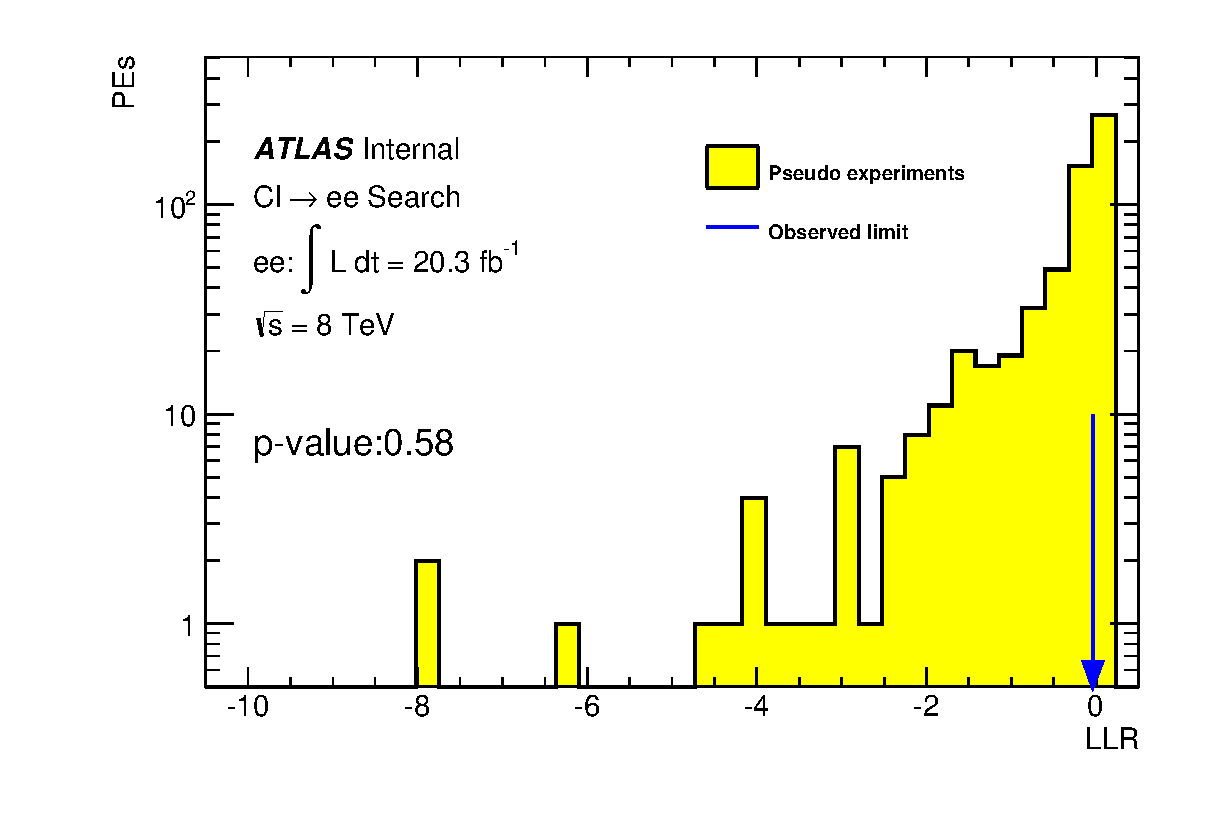
\includegraphics[width=0.49\linewidth]{images/ee__LL_minus_L2/LLR.eps}
            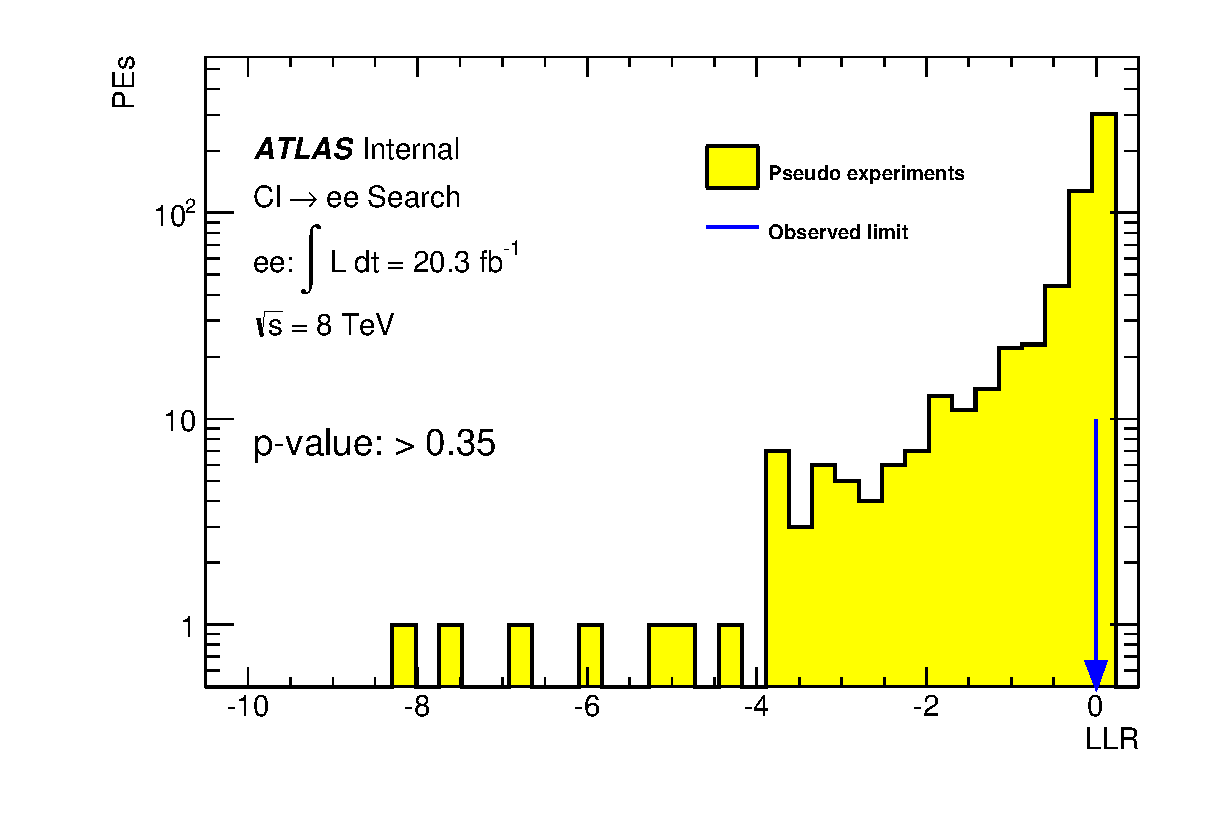
\includegraphics[width=0.49\linewidth]{images/ee__LR_minus_L2/LLR.eps}
        \end{center}
       \caption{Distribution of negative Log Likelihood Ratio's for the CI formalisms LL (left) and LR (right) with constructive interference given a uniform positive prior in $1/\Lambda^{2}$.}
       \label{fig:LLR_CI_main}
    \end{figure}

    % \begin{figure}[h]
    %     \begin{center}
    %         %\includegraphics[scale=0.6]{images/}
    %     \end{center}
    %    \caption{Distribution of negative Log Likelihood Ratio's for the ADD formalism GRW given a uniform positive prior in $1/M_{s}^{8}$.}
    %    \label{fig:LLR_ADD_main}
    % \end{figure}


    \begin {table}[h]
        \begin{center}
        \begin{tabular}{ | l | c | c | c | c | } 
            \hline
            \multirow{2}{*}{$p$-value [\%]} & \multicolumn{2}{c|}{1/$\Lambda^2$} & \multicolumn{2}{c|}{1/$\Lambda^4$} \\
            \cline{2-5}
            & Constructive & Destructive & Constructive & Destructive \\
            \hline
            LL: ee & 58 & 60 & $>$ 76 & $>$ 58 \\
            LR: ee & $>$ 35 & 36 & $>$ 85 & $>$ 62 \\
            RR: ee & $>$ 35 & 68 & $>$ 75 & $>$ 62 \\
            \hline
        \end{tabular}
        \caption{$p$-values for all CI formalisms and prior's.}
        \label{tab:pvalue_CI}
        \end{center}
    \end {table}


    \begin {table}[h]
        \begin{center}
        \begin{tabular}{ | l | c | c | c | } 
            \hline
            $p$-value [\%] & 1/M$_S^4$ & 1/M$_S^8$ \\
            \hline
            GRW: ee & 51 & $>$ 58 \\
            \hline
        \end{tabular}
        \caption{$p$-values for ADD with each prior.}
        \label{tab:pvalue_ADD}
        \end{center}
    \end {table}






\section{Setting Limits}
    
    With no sign of new physics found, limits are set on the lower value of the scale of new physics for each CI and ADD formalism. Limits in $\Theta$ are extracted from each of the 1000 PE's for each formalism and the mean of this distribution is taken as the expected limit and converted into a limit on $\Lambda$ for CI and M$_{s}$ for ADD. Figure \ref{fig:Theta_CI_main} shows the distribution of these PE's in $\Theta$ along with the mean value of the distribution taken as the expected limit. More of these distributions are found in appendix \ref{ap:stat}. Tables \ref{tab:limits_CI} and \ref{tab:limits_ADD} then show the expected limits converted into $\Lambda$ and M$_{s}$ respectively where the same procedure had been done in the ADD channel. The final observed limits are also included in these figures and tables compared to the expected limits and extracted from the observed data. The limits in the ADD search are also converted from the GRW formalism to all of the other formalism discussed in section \ref{sec:ADD_T} by a rearrangement of equation \ref{eq:ADDF}. The exception is the HLZ n = 2 formalism which has its own MC sample and limits are set in the same way as for GRW. The limits on all other formalisms discussed are then seen in \ref{tab:ADD_results_formalisms}.


    \begin{figure}[h]
        \begin{center}
            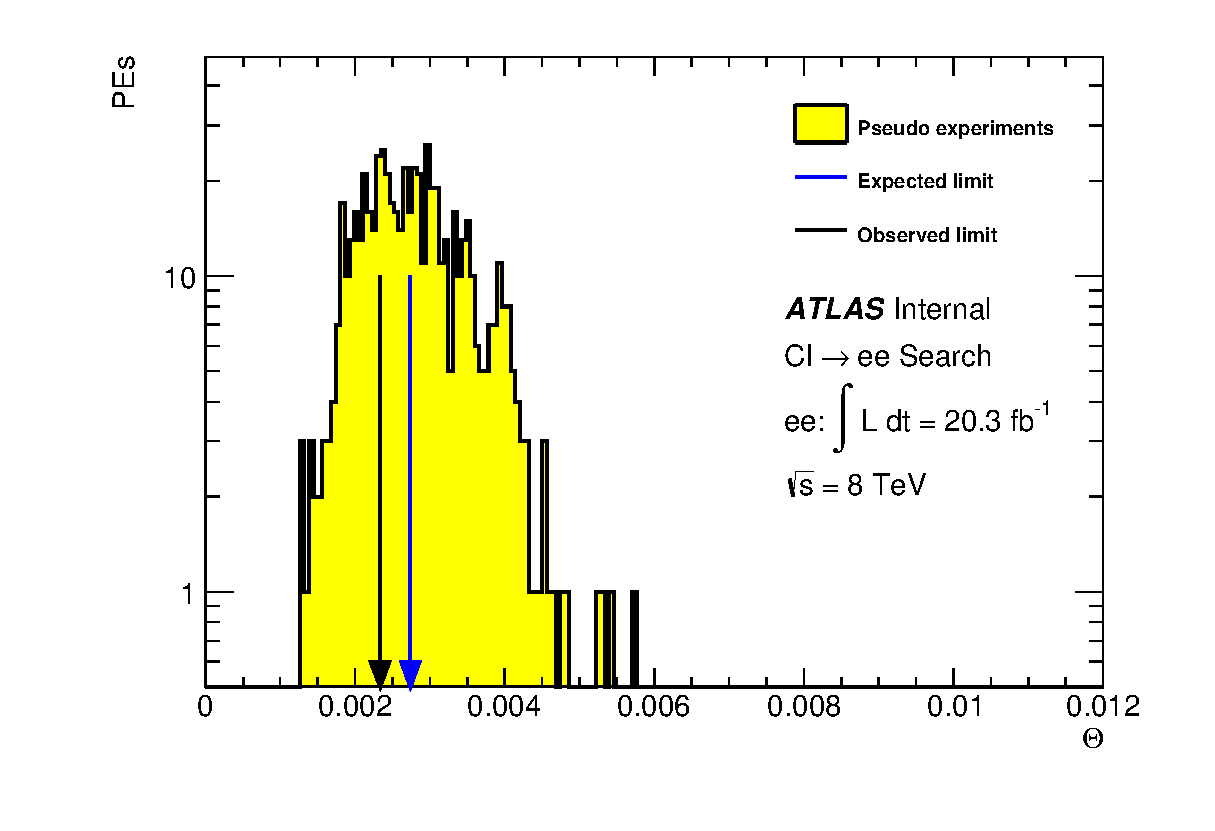
\includegraphics[width=0.49\linewidth]{images/ee__LL_minus_L2/Theta.eps}
            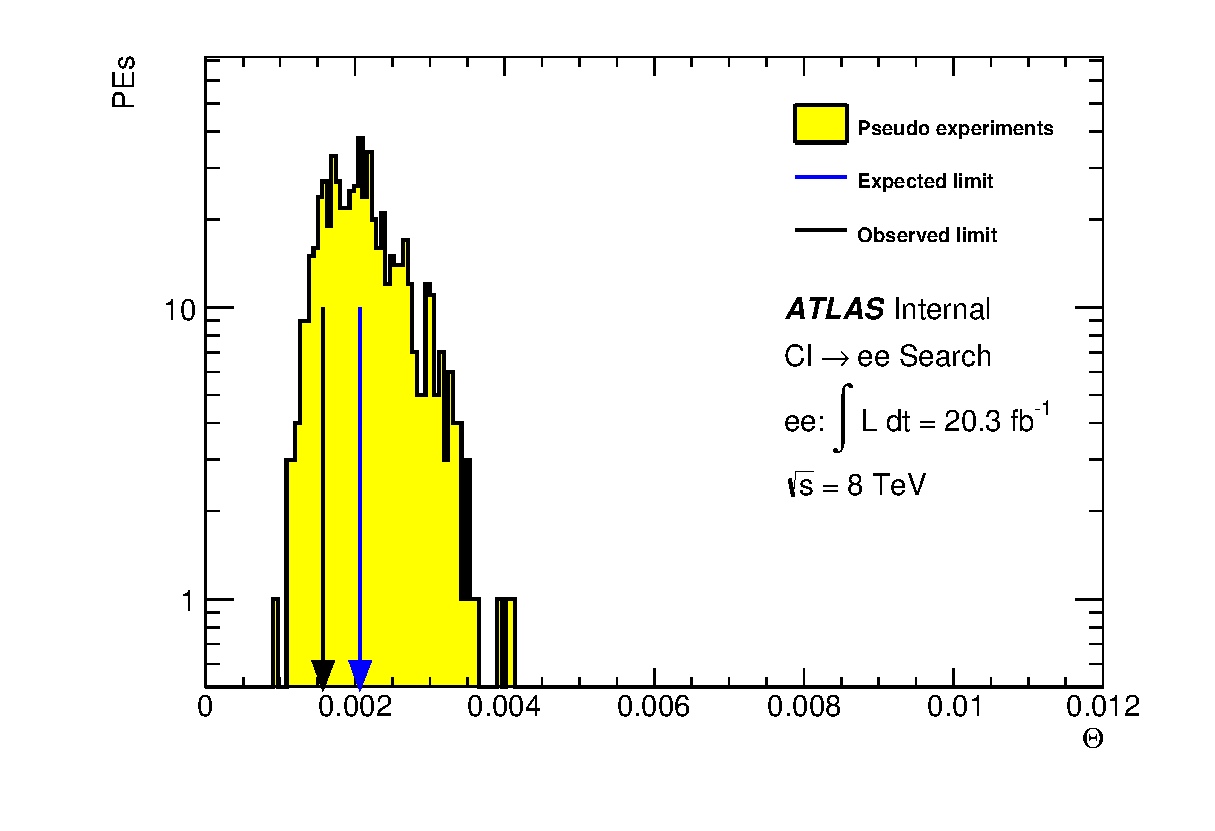
\includegraphics[width=0.49\linewidth]{images/ee__LR_minus_L2/Theta.eps}
        \end{center}
       \caption{Distribution of PE's with associated limits for CI formalisms LL (left) and LR (right) with constructive interference given a uniform positive prior in $1/\Lambda^{2}$. The mean value is shown as the expected limit for comparison to the observed limit shown. $\Theta$ = $1/\Lambda^{2}$}
       \label{fig:Theta_CI_main}
    \end{figure}

    % \begin{figure}[h]
    %     \begin{center}
    %         %\includegraphics[scale=0.6]{images/}
    %     \end{center}
    %    \caption{Distribution of PE's with associated Limits for the ADD formalism GRW given a uniform positive prior in $1/M_{s}^{8}$.}
    %    \label{fig:Theta_ADD_main}
    % \end{figure}



    \begin {table}[h]
        \begin{center}
        \begin{tabular}{  l | c | c | c | c  } 
            \hline
            \hline
            \multirow{2}{*}{Limits [TeV]} & \multicolumn{2}{c|}{1/$\Lambda^2$} & \multicolumn{2}{c}{1/$\Lambda^4$} \\
            \cline{2-5}
             & Constructive & Destructive & Constructive & Destructive \\
            \hline
            Expected LL: ee       & 19.11 & 14.02 & 17.44 & 13.02 \\
            Observed LL: ee       & 20.71 & 16.35 & 18.58 & 14.72 \\
            \hline
            Expected LR: ee       & 22.01 & 17.37 & 20.09 & 16.26 \\
            Observed LR: ee       & 25.16 & 19.19 & 22.19 & 17.68 \\
            \hline
            Expected RR: ee       & 18.97 & 14.23 & 17.23 & 13.14 \\
            Observed RR: ee       & 20.22 & 16.57 & 18.34 & 14.89 \\
            \hline
            \hline
        \end{tabular}
        \caption{Expected and observed 95\% C.L. lower limits for all CI formalisms and prior's.}
        \label{tab:limits_CI}
        \end{center}
    \end {table}


    \begin {table}[h]
        \begin{center}
        \begin{tabular}{ l | c | c } 
            \hline
            \hline
            GRW ADD Limits [TeV] & 1/M$_S^4$ & 1/M$_S^8$ \\
            \hline
            Expected: ee & 4.79 & 4.50 \\
            Observed: ee & 4.79 & 4.50 \\
            \hline
            \hline
        \end{tabular}
        \caption{Expected and observed 95\% C.L. lower limits for ADD with each prior.}
        \label{tab:limits_ADD}
        \end{center}
    \end {table}


\begin{table}[]
  \begin{center}
    \begin{tabular}{c|c|c|c|cccccc}
        \hline
        \hline
        \multicolumn{10}{c}{Expected and Observed Limit on $M_{S}$ [TeV]} \\
        \hline
        \multirow{2}{*}{Channel} & \multirow{2}{*}{Prior} & \multirow{2}{*}{GRW} & \multirow{2}{*}{Hewett} & \multicolumn{6}{c}{HLZ} \\
        \cline{5-10}
                &       &     &        & n= 2 &  n=3 & n=4 & n=5 & n=6 & n=7 \\
        \hline
        \hline
        Expected: $ee$      & \multirow{2}{*}{$1/M_{S}^{4}$} & 4.79 & 4.28 & 4.85 & 5.70 & 4.79 & 4.33 & 4.03 & 3.81 \\
        Observed: $ee$      &  & 4.79 & 4.28 & 4.86 & 5.70 & 4.79 & 4.33 & 4.03 & 3.81 \\
        \hline
        Expected: $ee$      & \multirow{2}{*}{$1/M_{S}^{8}$} & 4.50 & 4.25 & 4.42 & 4.90 & 4.50 & 4.27 & 4.12 & 4.01 \\
        Observed: $ee$      &  & 4.50 & 4.25 & 4.42 & 4.90 & 4.50 & 4.27 & 4.12 & 4.01 \\
        \hline
        \hline
    \end{tabular}
  \end{center}
    \caption{Expected and observed 95\% C.L. lower limits on $M_{S}$, for ADD signal in the GRW, Hewett and HLZ formalisms.
    \label{tab:ADD_results_formalisms}}
\end{table}



\section{Combination with the Muon Search}

    A similar analysis was carried out at the same time as this one looking at the dimuon decay channel instead. This analysis followed the same procedure and after failing to find any signals limits were set on the scale of new physics. Assuming lepton universality integrated luminosity can effectively be doubled by combining the results from both channels. Therefore the posterior pdf's from each analysis were combined in BAT and new limits set on the scale of new physics. Care was taken to correctly treat sources of systematic uncertainty that are correlated between analyses. Combined limits of this form can be found in tables \ref{tab:Comb_Limits_CI} and \ref{tab:Comb_Limits_ADD} for the CI and ADD models respectively while table \ref{tab:ADD_results_formalisms_comb} shows the combined limits for the other ADD formalisms. It can be seen that that limits do not increase to a large degree. This is due to two factors; on the whole muon limits are lower that electron limits due to a greater inefficiency in selecting muon candidates, also this analysis has started to reach the stage that it is not statistics limited and an increase in collision energy is required to push the limits higher. The muon invariant mass distribution can be seen in figure \ref{fig:invMass_muon} for comparison with the electron distribution. 

   \begin{figure}[h]
        \begin{center}
            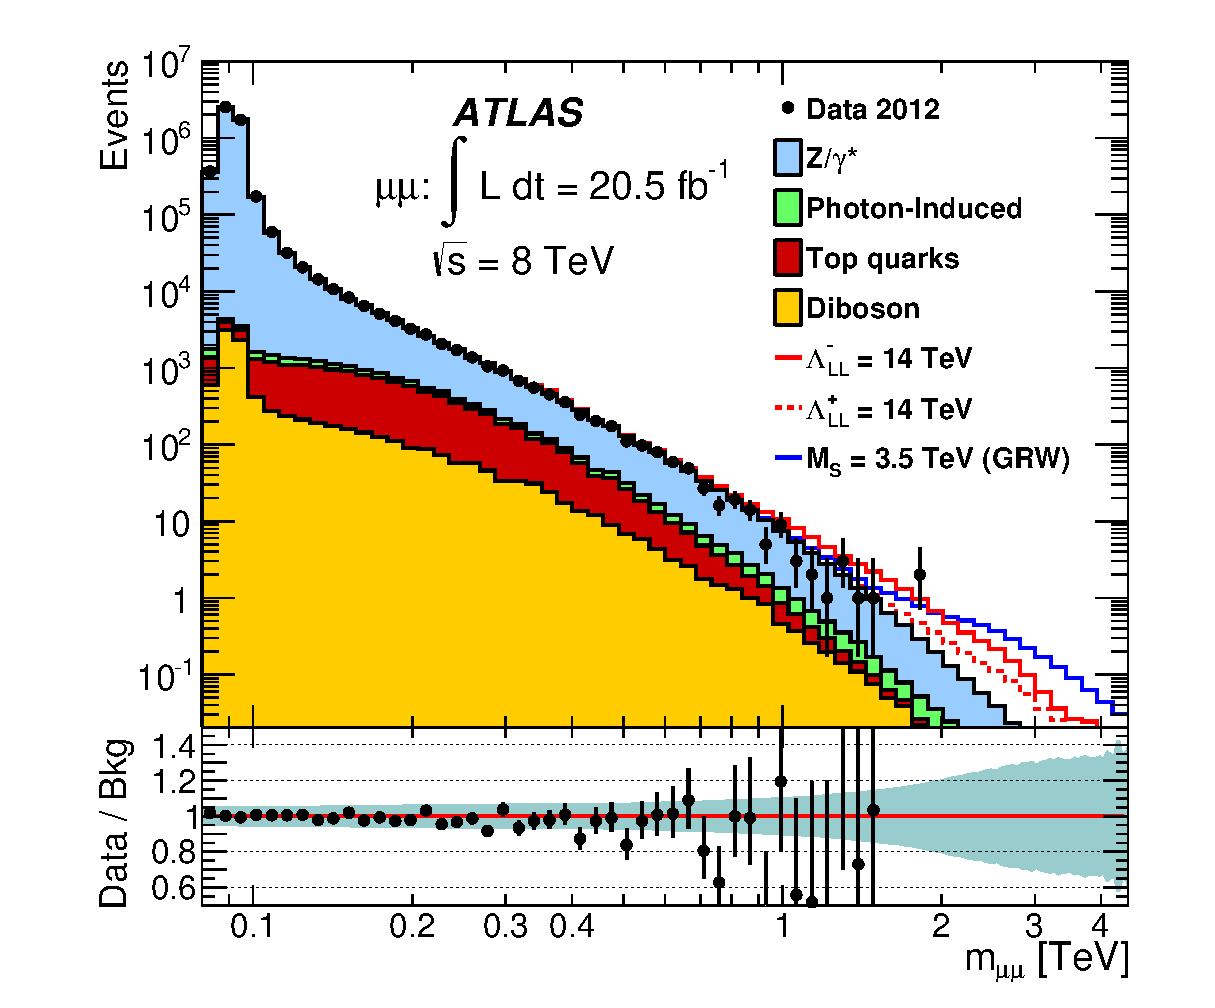
\includegraphics[width=0.8\linewidth]{images/fig_01b.eps}
        \end{center}
       \caption{Dimuon invariant mass comparison between data and MC with possible signal overlays of CI and ADD. Ratio between data and background included with band showing size of total background systematic. The distribution has bin width constant in $\log(M_{\mu\mu})$.}
       \label{fig:invMass_muon}
    \end{figure}


    The combined limits mark the highest limits set for this analysis owing to the higher effective luminosity. 


\begin{table}[p]
\centering
\begin{tabular}{ l|c|c|c|c }
    \hline
    \hline
    \multirow{2}{*}{Limits [TeV]} & \multicolumn{2}{c|}{1/$\Lambda^2$} & \multicolumn{2}{c}{1/$\Lambda^4$} \\
    \cline{2-5}
     & Constructive & Destructive & Constructive & Destructive \\
    \hline
    Expected LL: $\ell\ell$ & 21.44 & 19.11 & 14.73 & 13.81 \\
    Observed LL: $\ell\ell$  & 21.55 & 19.61 & 17.15 & 15.35 \\
    \hline
    Expected LR: $\ell\ell$ & 24.78 & 23.12 & 18.46 & 17.57 \\
    Observed LR: $\ell\ell$ & 26.25 & 23.77 & 18.95 & 17.79 \\
    \hline
    Expected RR: $\ell\ell$ & 20.98 & 19.11 & 14.99 & 14.21 \\
    Observed RR: $\ell\ell$ & 21.11 & 19.31 & 17.50 & 15.58 \\
    \hline
    \hline
\end{tabular}
\caption{Combined expected and observed 95\% C.L. lower limits for the 2D LL, LR, and RR Contact Interaction search using a uniform positive prior.}
\label{tab:Comb_Limits_CI}
\end{table}


\begin{table}[p]
\centering
\begin{tabular}{ l | c | c }
    \hline
    \hline
    GRW ADD Limits [TeV] & 1/M$_S^4$ & 1/M$_S^8$ \\
    \hline
    Expected: $\ell\ell$ & 4.83 & 4.60 \\
    Observed: $\ell\ell$ & 5.12 & 4.79 \\
    \hline
    \hline
\end{tabular}
\caption{Combined expected and observed 95\% C.L. lower limits for the ADD search using a uniform positive prior.}
\label{tab:Comb_Limits_ADD}
\end{table}




\begin{table}[]
  \begin{center}
    \begin{tabular}{c|c|c|c|cccccc}
        \hline
        \hline
        \multicolumn{10}{c}{Expected and Observed Limit on $M_{S}$ [TeV]} \\
        \hline
        \multirow{2}{*}{Channel} & \multirow{2}{*}{Prior} & \multirow{2}{*}{GRW} & \multirow{2}{*}{Hewett} & \multicolumn{6}{c}{HLZ} \\
        \cline{5-10}
                &       &     &        & n= 2 &  n=3 & n=4 & n=5 & n=6 & n=7 \\
        \hline
        \hline
        Expected: $\ell\ell$      & \multirow{2}{*}{$1/M_{S}^{4}$} & 4.83 & 4.31 & 5.09 & 5.74 & 4.83 & 4.36 & 4.06 & 3.84 \\
        Observed: $\ell\ell$      &  & 5.12 & 4.57 & 5.47 & 6.09 & 5.12 & 4.62 & 4.30 & 4.07 \\
        \hline
        Expected: $\ell\ell$      & \multirow{2}{*}{$1/M_{S}^{8}$} & 4.60 & 4.35 & 4.67 & 5.01 & 4.50 & 4.37 & 4.22 & 4.10 \\
        Observed: $\ell\ell$      &  & 4.79 & 4.53 & 4.94 & 5.23 & 4.79 & 4.56 & 4.40 & 4.27 \\
        \hline
        \hline
    \end{tabular}
  \end{center}
    \caption{Expected and observed combined 95\% C.L. lower limits on $M_{S}$, for ADD signal in the GRW, Hewett and HLZ formalisms.
    \label{tab:ADD_results_formalisms_comb}}
\end{table}



